\section{Experimental results}
\label{sec:experimental_results}
In this section, we present experimental results of the HF6 concept on low-cost sensor analytics applications. As a use case, we present a CNN-regression model to predict x- y- coordinates of structural anomalies based on acoustic sensor data. We compare quantitative and qualitative aspects of the data analytics using floating-point, fixed-point, and HF6 approach.

To demonstrate the HF6 hardware concept, we deploy the CNN model for low-power inference in the smallest Zynq SoC. We compare the performance of the dedicated hardware implemented with standard floating-point and HF6 architecture.

\subsection{Sensor Analytics Application}
The sensor analytics model is designed to predict x- y- coordinates of acoustic emissions on a metal plate with noise disturbance. We present the experimental setup, data sets, and the CNN-regression model.

\subsubsection{Experimental Setup}
The experiment uses eight piezoelectric sensors (Vallen Systeme VS900) fixed on a metal plate (90 cm x 86.6 cm x 0.3 cm). The VS900 devices can operate either in active or passive mode. Six VS900 are used in passive mode as acoustic sensors and two in active mode to produce acoustic emissions. These acoustic emissions represent the anomalies on x- y- coordinates and the noise disturbance of the system. See \fig{fig:data_set}(a). The acoustic emissions are labeled with their coordinates to create data sets.

\subsubsection{Data Sets}
The data sets are recorded with pulses and the x- y- coordinates as labels. The pulses for training and validation data sets are shown in \fig{fig:data_set}(b) and \fig{fig:data_set}(c), respectively. The pulses for training and validation data sets are mutually exclusive, this exclusion is represented by the cross symbols in \fig{fig:data_set}(c).

In order to create a reproducible acoustic emission, narrow-banded in the frequency domain, we use 9-cycle sine pulse in a Hanning window with central frequency $f_\mathrm{c}$. We assume guided Lamb waves based on the plate structure. The narrow-band behavior also reduces the dispersion of the acoustic emission waves~\cite{hannwindowsine}. The waveform can be expressed as a function of time $t$ as follows:

\begin{equation}
x_\mathrm{pulse}(t) = \frac{1}{2} \Big(1-\cos{\frac{f_\mathrm{c} t}{5}} \Big) A_0 \sin{f_\mathrm{c} t}.
\end{equation}

In order to generate the data sets, we use slightly different pulse amplitudes and frequencies for excitation. The pulse frequency $f_c$ is varied in 1 kHz steps between 300 kHz and 349 kHz and the amplitude $A_0$ is varied in 0.1 V steps between 2.6 V and 3.5 V. This results in 500 different pulses for each of the excitation points. \fig{fig:data_set}(c) illustrates the grid layout used to collect samples for the data sets. This grid is 10 by 10 and it does not consider the four corners as they are used for structure holders.

The labeled pulses and the noise disturbance signals are generated by arbitrary waveform generators (AWGs). The sensor signals are recorded via a Vallen AMSY-6 measurement system with a resolution of 18 bits and a sampling rate of $f_\mathrm{S} = 10 MHz$. The noise disturbance is a gaussian noise signal with amplitudes between 0-3 V. This noise is applied via the piezoelectric device $N$ at $x=0.227$ and $y=0.828$, see \fig{fig:data_set}(a).

In order to obtain both time and frequency domain information, the acquired pulses are converted into the time-frequency domain using the Short-Time Fourier Transform (STFT). It is calculated as follows~\cite{stft_lit}:

\begin{flalign}
\label{stft_eq2}
\mathcal{F}_{m,k}^\gamma= \sum_{n=0}^{N-1} x[n] \cdot \gamma^*[n-m\Delta M]\cdot \mathrm{e}^{\frac{-j 2 \pi k n }{N}}
\end{flalign}

Here $x[n]$ describes a discrete-time signal and $\gamma^*[n-m\Delta M]\cdot \mathrm{e}^{\frac{-j 2 \pi k n }{N}}$ the time- and frequency-shifted window function inside the considered interval $[0 , N-1]$. $\Delta M$ describes the time shift and $N$ the transformation window. Since only discrete frequencies and time points are considered, $m = 0,1,...,M-1$ is valid. This complex-valued STFT is converted to real numbers via the magnitude square for pictorial representation in a spectrogram $\mathcal{S}_{m,k}$:

\begin{flalign}
\label{stft_eq3}
\mathcal{S}_{m,k}= \left|\mathcal{F}_{m,k}^\gamma\right|^2 = \left|\sum_{n=0}^{N-1} x[n] \cdot \gamma^*[n-m\Delta M]\cdot \mathrm{e}^{\frac{-j 2 \pi k n }{N}} \right|^2
\end{flalign}

In addition, the spectrograms used are scaled in decibels. The spectrogram in decibels $\mathcal{S}_{m,k,\mathrm{dB}}$ results in $\mathcal{S}_{m,k,\mathrm{dB}}= 20 \cdot \mathrm{log}_{10}(\mathcal{S}_{m,k})$. For the conversion of the data a signal length of 400 \textmu s (75 \textmu s pretrigger and 325 \textmu s post trigger) is used. Thus, the arrival times of the pulses are included in the spectrogram for all channels and labeled positions. A Blackman window function~\cite{blackman_window}, a Fast Fourier Transform (FFT) length of 32 samples, and an overlap of 8 samples are used. The spectrograms are calculated for frequencies in the range of 100 kHz to 500 kHz. This results in a spectrogram with 8x16 values (8 frequency values, 16 time values). In addition to the original 400 \textmu s windows, four further variants with time shifts of 15 \textmu s/ 30 \textmu s/ 45 \textmu s/ 60 \textmu s were calculated in order to generate larger data sets. Subsequently, all spectrograms were converted to grayscale with scaling between -100dB and -40dB, see \fig{fig:spectrograms}. Overall, the data set has a size of 500 (pulses) $\cdot$ 5 (spectrograms) $\cdot$ 6 (listening sensors) $\cdot$ 96 (excitation points) = 1,440,000 images.

\begin{figure}[t!]
	\centering
	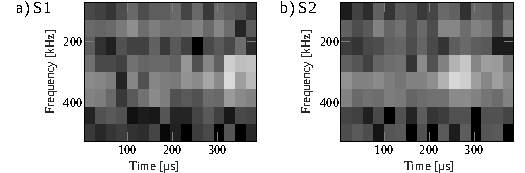
\includegraphics[width=\columnwidth]{../figures/histograms/spectrograms.pdf}
	\caption{Spectrograms of sensors $S_1, S_2$ converted to grayscale for pulses at $x =0.105$, $y = 0.109$ with noise disturbance.}
	\label{fig:spectrograms}
\end{figure}

\begin{figure}[t!]
	\centering
	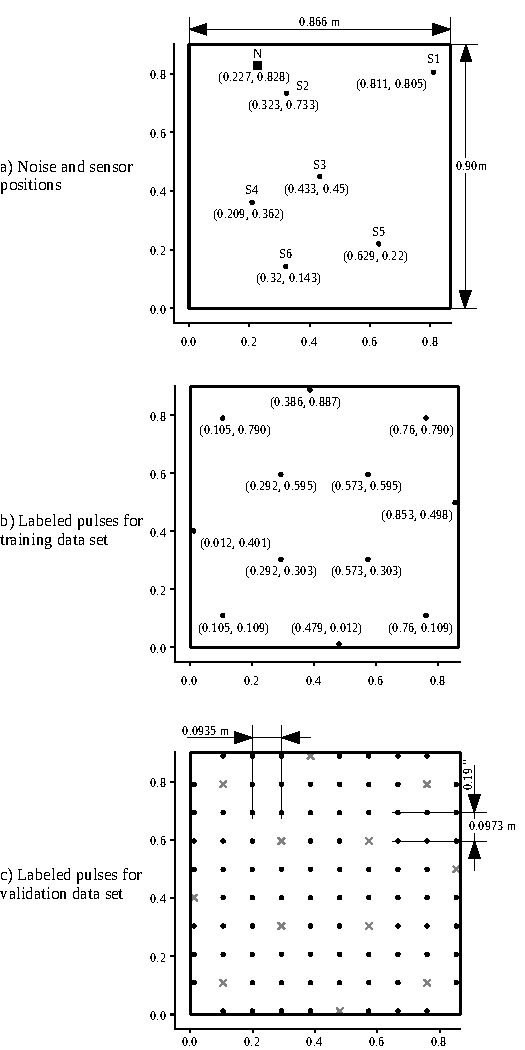
\includegraphics[width=\columnwidth]{../figures/histograms/data_set.pdf}
	\caption{(a) Illustrates the Sampling layout for training and validation data set.}
	\label{fig:data_set}
\end{figure}

\subsubsection{CNN-Regression Model}
The data analytics is implemented with a CNN-regression model, see \fig{fig:model}. The structure of the model is described below:

\begin{enumerate}[label=\alph*)]
\item Input patterns. This is an input tensor composed of spectrograms from the sensor signals. The tensor shape is defined by $S \times T \times F$, where $S$ is the number of sensors, and $T \times F$ is the time-frequency resolution of the spectrograms, see \fig{fig:model}(a).

\item Feature extraction. This is composed of three blocks of convolution, batch normalization, and max-pooling layers, see \fig{fig:model}(b). The number of channels in the convolution layers are defined by the hyper-parameters $A$, $B$, and $C$.

\item Regression function. This is an arbitrary function implemented with two fully connected layers and an output layer with linear activation, see \fig{fig:model}(c).
\end{enumerate}


\begin{figure*}[t!]
	\centering
	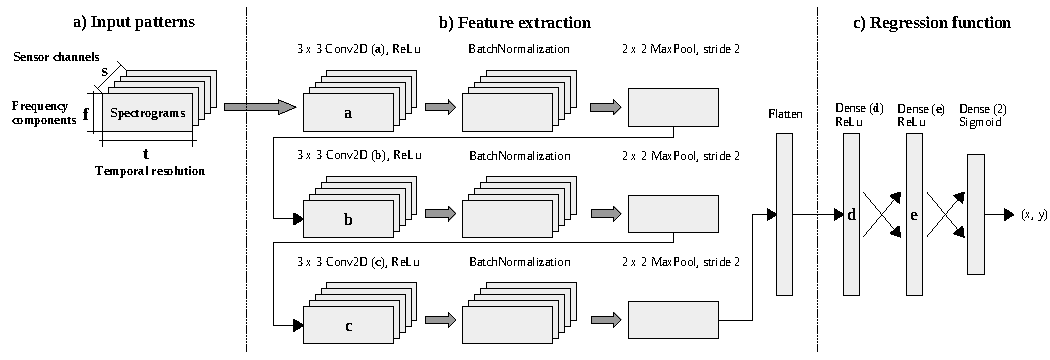
\includegraphics[width=\textwidth]{../figures/model.pdf}
	\caption{CNN model for sensor analytics.}
	\label{fig:model}
\end{figure*}


\subsection{Training}
\subsubsection{Training with Iterative Early Stop}
The model in \fig{fig:model} is trained using Adam algorithm with iterative early stop, described in \Algo{alg:training}. The Adam optimizer is configured with the default settings presented in \cite{kingma2014adam}: $\alpha = 0.001$, $\beta_1 = 0.9$, $\beta_2 = 0.999$, and $\epsilon = 1\mathrm{e}{-8}$. The optimizer is executed with early stop patience of 10 epochs and mini-batch size of 512 samples. The training cycle aborts with patience of 10 search iterations.

The training results are illustrated in \fig{fig:optimization}. The initial model is obtained at the first early stop. Each stop initializes the moving averages of the Adam optimization. In subsequent iterations, the model is updated when better minimum is reached.

For the initial model, the first stop takes 43 epochs and subsequent iterations take from 13 to 17 epochs. The training time is 216 minutes (NVIDIA GeForce RTX 3050). The initial and final models obtain $MSE = 0.0135 m^2$ and $MSE=0.0122m^2$, respectively. This represents a reduction of $9.62\%$ in the MSE.

\begin{figure}[t!]
	\centering
	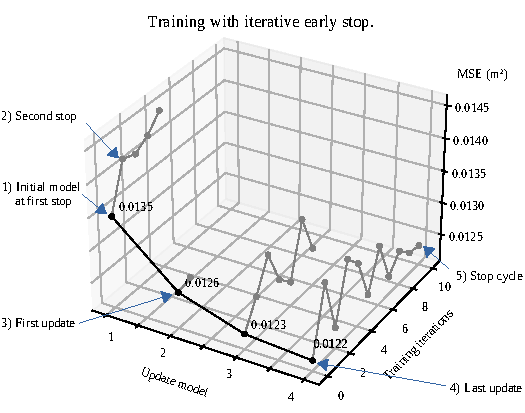
\includegraphics[width=\columnwidth]{../figures/histograms/optimization.pdf}
	\caption{Training with iterative early stop.}
	\label{fig:optimization}
\end{figure}

\subsubsection{Quantized Aware Training}
The HF6 quantization is applied on the base model as a post-training step. \fig{fig:optimization} shows the HF6 quantization applied to the base model. This minimizes the inference loss with 6-bit floating-point quantization on the trainable parameters of convolution layers.
\begin{figure}[h!]
	\centering
	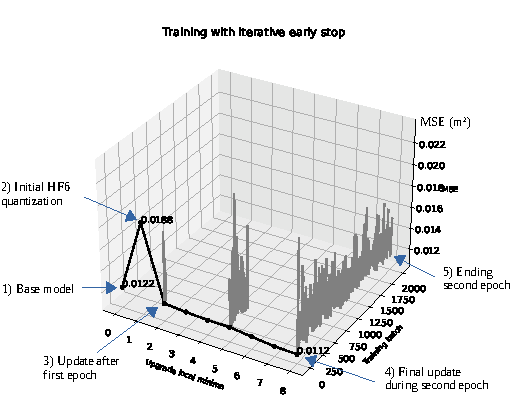
\includegraphics[width=\columnwidth]{../figures/histograms/optimization_E4M1.pdf}
	\caption{Training with iterative early stop.}
	\label{fig:optimization_E4M1}
\end{figure}

\begin{figure*}[t!]
	\centering
	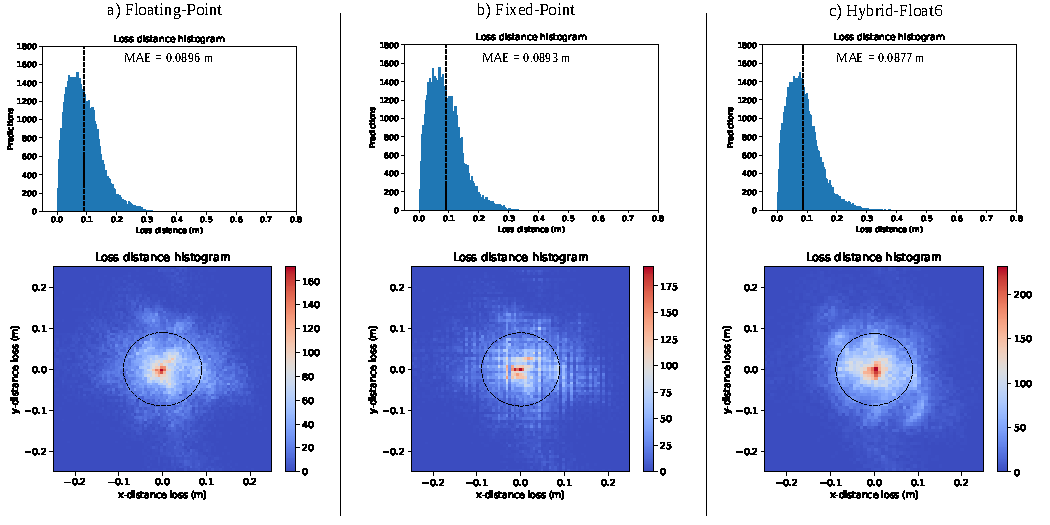
\includegraphics[width=\textwidth]{../figures/histograms/model_evaluation.pdf}
	\caption{CNN model for case study.}
	\label{fig:model_evaluation}
\end{figure*}

\begin{figure}[t!]
	\centering
	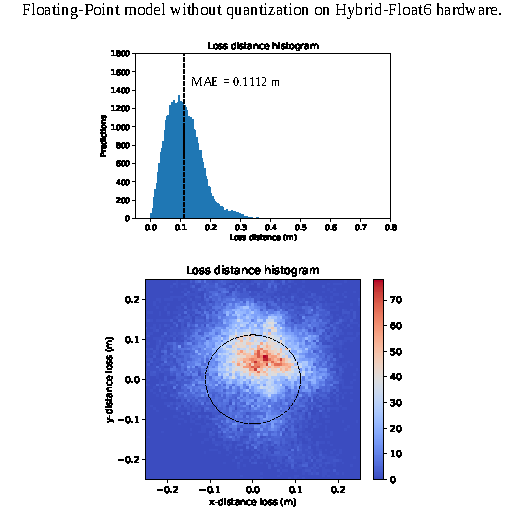
\includegraphics[width=\columnwidth]{../figures/histograms/model_evaluation_wo_quant.pdf}
	\caption{CNN model for case study.}
	\label{fig:model_evaluation_wo_quant}
\end{figure}

\subsection{Hardware Design Exploration}
The proposed hardware/software co-design is demonstrated on the Zynq-7007S system-on-chip (SoC) in the MiniZed development board. This device integrates a single ARM Cortex-A9 processing system (PS) and programmable logic (PL) equivalent to Xilinx Artix-7 (FPGA) in a single chip \cite{xilinx2015zynq}. The Zynq-7007S SoC architecture maps the custom logic and software in the PL and PS respectively as an embedded system.

In this platform, we implement the proposed hardware architecture to deploy the \REVIEWR{CNN model} for \REVIEWR{SHM} shown in \Fig{fig:models}. The CNN model is created, trained, and quantized using Keras/TensorFlow with Python on a desktop computer. The resulting model is converted to TensorFlow Lite, which is deployed on the MiniZed. The Zynq-7007S SoC performs the model inference with TensorFlow Lite core API running on the PS. The computational workload of the convolution layers is delegated to the TP on the PL.

\subsection{Performance benchmark}
\subsubsection{Benchmark on embedded CPU}

We examine the performance of the embedded CPU for inference with no hardware acceleration. In this case, the embedded software builds the CNN as a sequential model mapping the entire computation to the CPU (ARM Cortex-A9) at 666 MHz and a power dissipation of \REVIEWR{$1.658 W$}.

The inference on the CPU achieves a latency of \REVIEWR{$40 ms$}. The model is computed with standard floating-point arithmetic with no accuracy degradation. The latency and schedule of the CNN inference are displayed in \Tab{tab:latency_sw} and \fig{fig:latency_sw} respectively.

\subsubsection{Benchmark on tensor processor with standard floating-point computation}
To benchmark the computation on hardware TP with standard floating-point, we implement the system architecture with one TP. In this case, the embedded software builds the CNN as a sequential model mapping \emph{Conv2D} tensor operations to the TP at 200 MHz as clock frequency. The hardware mapping and the computation schedule of this deployment are displayed in \Tab{tab:latency_fp} and \fig{fig:latency_pu_fp}.

The post-implementation resource utilization and power dissipation are shown in \Tab{tab:resource_fp}.

The TP instantiates an on-chip weight matrix of \REVIEWR{$52,000$} entries, wish is sufficient to store \REVIEWR{$W\in\mathbb{R}^{5\times 5\times 2\times 32}$} and $B\in\mathbb{R}^{5\times 5\times 32\times 64}$ for weight and bias, respectively. In order to reduce BRAM utilization, we use a custom floating-point representation composed of 4-bit exponent and 4-bit mantissa. Each 8-bit entry is promoted to its standard floating-point representation for computation.


\REVIEW{The implementation of dot-product with standard floating-point arithmetic (IEEE 754) utilizes proprietary multiplier and adder floating-point operator cores. Vivado HLS accomplishes floating-point arithmetic operations by mapping them onto Xilinx LogiCORE IP cores, these floating-point operator cores are instantiated in the resultant RTL\mbox{\cite{hrica2012floating}}. In this case, the implementation of the dot-product with the standard floating-point computation reuses the multiplier and adder cores already instantiated in other compute sections of the TP. The post-implementation resource utilization and power dissipation of the floating-point operator cores are shown in {\Tab{tab:LogiCORE}}.}

\begin{table}[!h]\centering
	\caption{Resource utilization and power dissipation of multiplier and adder floating-point (IEEE 754) operator cores.}\label{tab:LogiCORE}
	\scriptsize
	\begin{tabular}{lrrrrrr}\toprule
		\textbf{Core operation} &\textbf{DSP} &\textbf{FF} &\textbf{LUT} &\textbf{Latency (clk)} &\textbf{Power (mW)} \\\midrule
		Multiplier &3 &151 &325 &4 &7 \\
		Adder &2 &324 &424 &8 &6 \\
		\bottomrule
	\end{tabular}
\end{table}


\begin{table}[!htp]\centering
	\caption{Performance of the CPU and TP on each CONV\_2D tensor operation, computational cost, latency, throughput, power efficiency, and energy consumption.}\label{tab:performance}
	\scriptsize
	\begin{tabular}{lrrrrrr}\toprule
		\textbf{Operation} &\textbf{MFLOP} &\textbf{t (ms)} &\textbf{MFLOP/s} &\textbf{MFLOP/s/W} &\textbf{EDP (mJ)} \\\midrule
		& &\multicolumn{4}{l}{\textbf{a) CPU @666MHz, 1.187 W}} \\
		(1) CONV\_2D &0.691 &112.24 &6.16 &5.19 &133.23 \\
		(2) CONV\_2D &1.584 &213.13 &7.43 &6.26 &252.99 \\
		(3) CONV\_2D &0.475 &46.59 &10.20 &8.59 &55.31 \\
		& &\multicolumn{4}{l}{\textbf{b) TP Floating-Point @200MHz, 85 mW}} \\
		(1) CONV\_2D &0.691 &12.49 &55.34 &651.11 &1.06 \\
		(2) CONV\_2D &1.584 &16.39 &96.66 &1,137.20 &1.39 \\
		(3) CONV\_2D &0.475 &3.59 &132.44 &1,558.13 &0.30 \\
		& &\multicolumn{4}{l}{\textbf{c) TP Hybrid-Float6 @200MHz, 84 mW}} \\
		(1) CONV\_2D &0.691 &6.92 &99.81 &1,188.24 &0.58 \\
		(2) CONV\_2D &1.584 &4.41 &358.94 &4,273.09 &0.37 \\
		(3) CONV\_2D &0.475 &0.99 &482.44 &5,743.29 &0.08 \\
		\bottomrule
	\end{tabular}
\end{table}


\begin{table}[!htp]\centering
	\caption{Resource utilization and power dissipation on the Zynq-7007S SoC.}\label{tab: }
	\scriptsize
	\begin{tabular}{lrrrrrr}\toprule
		\multirow{2}{*}{\textbf{Platform}} &\multicolumn{4}{c}{\textbf{Post-implementation resource utilization}} &\multirow{2}{*}{\textbf{Power (W)}} \\\cmidrule{2-5}
		&\textbf{LUT} &\textbf{FF} &\textbf{DSP} &\textbf{BRAM 36Kb} & \\\midrule
		\multirow{2}{*}{Floating-Point} &5,578 &8,942 &23 &41.5 &\multirow{2}{*}{1.429} \\
		&39\% &31\% &35\% &83\% & \\
		\multirow{2}{*}{Hybrid-Float6} &7,313 &10,330 &20 &15 &\multirow{2}{*}{1.424} \\
		&51\% &36\% &30\% &30\% & \\
		\bottomrule
	\end{tabular}
\end{table}



\subsection{Design exploration with hybrid custom floating-point and logarithmic approximation}

In this section, we address a design exploration to evaluate our approach for inference using hybrid custom floating-point and logarithmic approximation. First, we examine the weight matrix of each convolution layer in order to determine the minimum requirements for numeric representation and memory storage. Second, we implement the TP using the minimal floating-point and logarithmic representation as design parameters. Finally, we evaluate the overall performance, inference accuracy, resource utilization, and power dissipation.

\subsubsection{Parameters for numeric representation of weight matrix}
\label{sec:parameters}
We obtain information for the numerical representation of the synaptic weight matrices from their $\log_2$-histograms presented in {\fig{fig:log2histogram}}. These histograms show the distribution of weight values in each matrix. We observe that the minimum integer exponent value is \REVIEWR{$-13$}. Hence, applying \REVIEWR{\equ{eq:exp_max}} and \REVIEWR{\equ{eq:bits_exp}} to the given CNN, we obtain \REVIEWR{$E_{\min}=-13$ and $N_E=4$}, respectively. Therefore, 4-bits are required for the absolute binary representation of the exponents.

For quality configurability, the mantissa bit-width is a knob parameter that is tuned by the designer. This procedure leverages the builtin error-tolerance of neural networks and performs a trade-off between resource utilization and QoR. In the following subsection, we present a case study with 1-bit mantissa corresponding to the custom floating-point approximation.

\subsubsection{Design exploration for dot-product with hybrid custom floating-point approximation}
For this design exploration, we use a custom floating-point representation composed of 4-bit exponent and 1-bit mantissa. This format is used for both the filter matrix and bias vectors of each convolution layer. The TP instantiates on-chip stationary both the filter matrix and bias vectors for \REVIEWR{$X$ and $Y$} entries of 6-bit (S1E4M1). The available memory size is large enough to store \REVIEWR{$W\in\mathbb{R}^{5\times 5\times 2\times 32}$ and $W\in\mathbb{R}^{5\times 5\times 32\times 64}$} for \REVIEWR{$\vec{F}$ and $\vec{b}$}, respectively. The hardware mapping and the computation schedule of this implementation are displayed in \Tab{tab:latency_cfp} and \Fig{fig:latency_pu_cfp_cycle}.

As shown in the computation schedule in \Tab{tab:latency_cfp} and \Fig{fig:latency_pu_cfp_cycle}, this implementation achieves a peak acceleration of \REVIEWR{55x}, and a power efficiency of \REVIEWR{5.5 GFLOP/s/W}. This configuration achieves an accuracy of \REVIEWR{$90.97\%$} correct regressions on the \REVIEWR{500} validation samples. This indicates an accuracy gain of \REVIEWR{$0.33\%$}.

The post-implementation resource utilization and power dissipation are shown in \Tab{tab:resource_cfp}.


\subsubsection{Design exploration for dot-product whit hybrid logarithmic approximation}
As the most efficient setup and yet the worst-case quality configuration, we use a 4-bit integer exponent for logarithmic representation of \REVIEWR{$\vec{F}$ and $\vec{b}$}. The hardware mapping and the computation schedule of this implementation are displayed in \Tab{tab:latency_log} and \Fig{fig:latency_pu_log_cycle}. As shown in the computation schedule in \Tab{tab:latency_log} and \Fig{fig:latency_pu_log_cycle}, this implementation achieves a peak acceleration of \REVIEWR{55X} and a power efficiency of \REVIEWR{5.5 GFLOPS/s/W}. This quality configuration achieves an accuracy degradation \REVIEWR{$0.84\%$} on correct regressions on the \REVIEWR{500} validation samples.

The post-implementation resource utilization and power dissipation are shown in \Tab{tab:resource_log}.

\begin{figure}[t!]
	\centering
	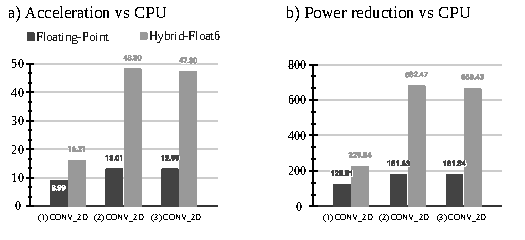
\includegraphics[width=1\columnwidth]{../figures/power_breakdown/acceleration_power_reduction.pdf}
	\caption{Acceleration and power reduction of the TP with floating-point and HF6 vs. CPU on the Zynq-7007S SoC.}
	\label{fig:ACCELERATION}
\end{figure}

\begin{figure}[t!]
	\centering
	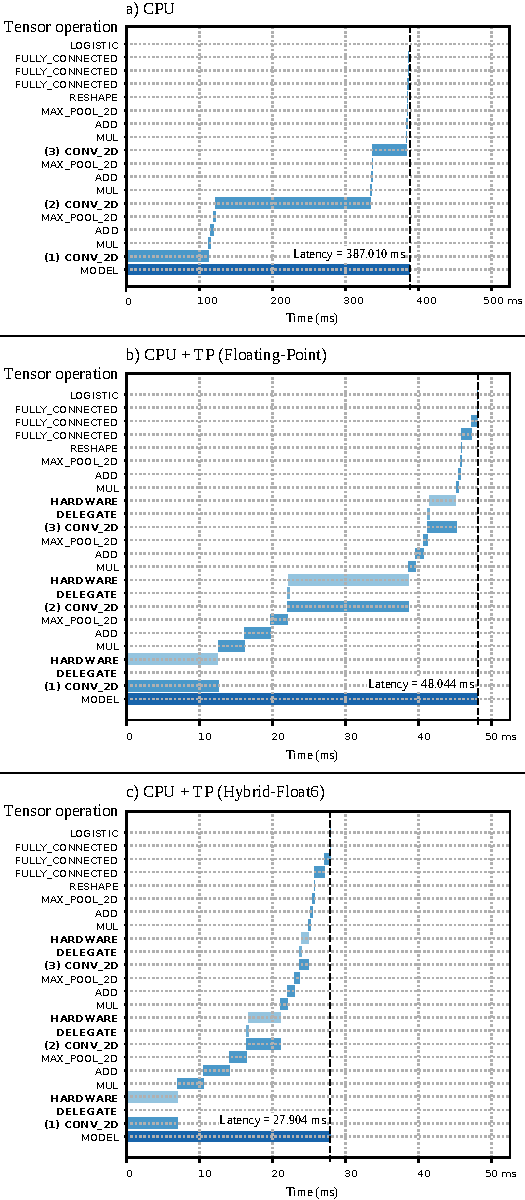
\includegraphics[width=1\columnwidth]{../figures/runtime/runtime.pdf}
	\caption{Inference run-time of TensorFlow Lite on the embedded system. (a) CPU ARM Cortex-A9 at 666MHz, (b) cooperative CPU + TP with floating-point Xilinx LogiCORE IP at 200MHz, and (c) cooperative CPU + TP with Hybrid-Float6 at 200MHz.}
	\label{fig:runtime}
\end{figure}

\begin{figure}[t!]
	\centering
	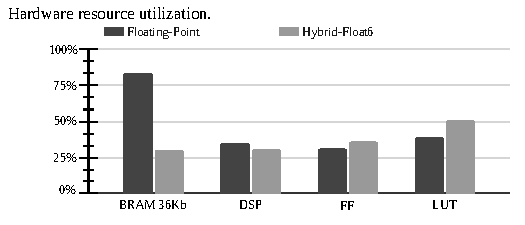
\includegraphics[width=1\columnwidth]{../figures/power_breakdown/resource_utilization.pdf}
	\caption{Hardware resource utilization on the Zynq-7007S SoC.}
	\label{fig:resource_utilization}
\end{figure}

\begin{figure}[t!]
	\centering
	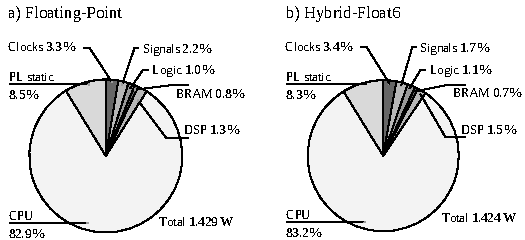
\includegraphics[width=1\columnwidth]{../figures/power_breakdown/power_breakdown.pdf}
	\caption{Estimated power dissipation on the Zynq-7007S SoC with PS at 666MHz and PL at 200MHz.}
	\label{fig:power}
\end{figure}

\subsection{Results and discussion}
As a reference, the inference on embedded CPU using standard 32-bit floating-point achieves an accuracy gain of \REVIEWR{0.3\%} with a latency of \REVIEWR{3,450.28ms}. As a second reference point, the inference on TP with standard floating-point presents a latency of \REVIEWR{34.5ms}, as result we get a $10.7\times$ latency enhancement.

As a demonstration of the proposed hardware/software architecture, the inference with TP using 5-bit custom floating-point (4-bit exponent, 1-bit mantissa) and 4-bit logarithmic (4-bit exponent) achieves \REVIEWR{$55.5\times$} latency enhancement. This results in an accuracy gain of \REVIEWR{$0.33\%$} and degradation of \REVIEWR{$0.46\%$}, respectively.

Regarding resource utilization and power dissipation, the TP with 5-bit custom floating-point has a \REVIEWR{$43.24\%$} reduction of BRAM, and a \REVIEWR{$12.35\%$} of improvement in energy efficiency over the standard floating-point implementation. \REVIEW{However, the hybrid dot-product with custom floating-point does not reuse the available floating-point operator cores instantiated from other computational sections (see {\Tab{tab:LogiCORE}}). Therefore, the logic required for the dot-product must be implemented, which is reflected as additional utilization of LUT and FF resources.} The experimental results of the design exploration are summarized in \Tab{tab:results}. \REVIEW{The platform implementations are summarized in \mbox{\Tab{tab:platform_comparison}}, and their power dissipation breakdowns are presented in {\fig{fig:platform_power_dissipation_breakdown}}.}


\subsection{Hardware design exploration}
To evaluate the methodology, we employ \Equ{eq:channel_in_memory}, giving the maximum hyper parameters from models $A$ and $B$: $W_{I}=32$, $C_{I}=60$, $C_{O}=120$, $K_{W} = K_{H} =3$. For the number formats, $BitSize_{I}=32$-b, and $BitSize_{F} = BitSize_{B}=6$-bits. To determine $V_{M}$, we use HLS tool, which gives an estimate of 6 RAM blocks. The performance evaluation and the hardware resource utilization are displayed in \tab{tab:perf} and \tab{tab:resource}, respectively.

\begin{enumerate}
\item{\textbf{XC7Z007S}}: As a resource-limited FPGA, this device has a capacity of 14,400 LUTs and 1.8Mb of BRAM. This limitation allows to instantiate one TP with \emph{Conv} due to its LUT capacity. With \Equ{eq:tp_memory}, we obtain a BRAM utilization of 789.84Kb. This implementation presents a peak runtime acceleration of $55\times$ in model $A$ at the tensor operation \emph{(3A) Conv} with a power reduction of $808\times$.

\item{\textbf{XC7Z010}}: This device has a capacity of 17,600 LUTs and 2.1Mb of BRAM. These resources allow to instantiate two TPs with \emph{Conv}, and one TP with \emph{Conv} and \emph{DConv} engines. With \Equ{eq:tp_memory}, we obtain a BRAM utilization of 1,580Kb. This implementation presents a peak runtime acceleration of $105\times$ in model $A$ at the tensor operation \emph{(3A) Conv} with a power reduction of $1121\times$. On model $B$, \emph{(6B) Conv} presents a peak acceleration of $43.8\times$. The \emph{DConv} tensor operator yields an acceleration of $6.75 \times$, which is limited since the pipelined vector dot-product performs on channel wise.
\end{enumerate}

